\documentclass{beamer}

\usepackage[utf8]{inputenc}
\usepackage{default}
\usepackage{listings}
\usepackage{hyperref}
\usepackage{graphicx}

\lstset{ %
  %backgroundcolor=\color{background},   % choose the background color; you must add \usepackage{color} or \usepackage{xcolor}
  basicstyle=\small\ttfamily,        % the size of the fonts that are used for the code
  %commentstyle=\color{mygreen},    % comment style
  frame=lines,                    % adds a frame around the code
  columns=fixed,
  keywordstyle=\color{blue},       % keyword style
  language=OCL,                 % the language of the code
  numbers=left,                    % where to put the line-numbers; possible values are (none, left, right)
  numbersep=5pt,                   % how far the line-numbers are from the code
  %numberstyle=\scriptsize\color{mygray}, % the style that is used for the line-numbers
  showspaces=false,                % show spaces everywhere adding particular underscores; it overrides 'showstringspaces'
  showstringspaces=false,          % underline spaces within strings only
  showtabs=false,                  % show tabs within strings adding particular underscores
  %stringstyle=\color{mymauve},     % string literal style
  tabsize=2                       % sets default tabsize to 2 spaces
}

\begin{document}

\author{Kristof Meixner \\ Sebastian Geiger}
\date{6 Mai 2014}
\title{fUML Refactoring with EMF\\\small{Business Informatic Group}}

\setbeamertemplate{navigation symbols}{%
    \usebeamerfont{footline}%
    \usebeamercolor[fg]{footline}%
    \insertframenumber/\inserttotalframenumber%
    \vspace{2mm}
    \hspace{1mm}
}

\begin{frame}
 \maketitle
\end{frame}


\begin{frame}
 \frametitle{Overview}

%TODO: 25 slides


\begin{itemize}
 \item Refactoring Overview
 \item UML Models and Refactoring
 \item Semantic Preservation
 \item Insurance Company Example
 \item fUML Introduction
 \item fUML Refactoring
 \item Refactoring Constraints with OCL
 \item Toolchain
 \item EMF Refactor
\end{itemize}

\end{frame}

\begin{frame}[fragile]
\frametitle{Refactoring Overview}
\begin{itemize}
 \item What is refactoring?
 \begin{itemize}
  \item ``defines a set of program restructuring operations'' that ``preserve the behavior of a program'' \cite{mast:REFOOF}
 \end{itemize}
 \item Why do we need it?
 \begin{itemize}
  \item Increases software and/or model quality
  \item Ensures reusability of components
  \item Supports change management in software lifecycle
 \end{itemize}
 \item Examples: rename class, extract superclass, encapsulate field.
 \item Detailed catalogues with refactorings exist (e.g. \cite{fow99})
\end{itemize}

\end{frame}

\begin{frame}
 \frametitle{UML Repetition}
 \begin{itemize}
  \item Unified Modeling Language (v2.4.1) standardized by Object Management Group \cite{man:UML}
  \item General-purpose modeling language in the field of software engineering (Wikipedia)
  \item Includes different diagram types for architecture structure \& behavior
  \item Allows contraint definition via OCL \cite{man:OCL}
 \end{itemize}
\begin{figure}[h!t]
 \centering
 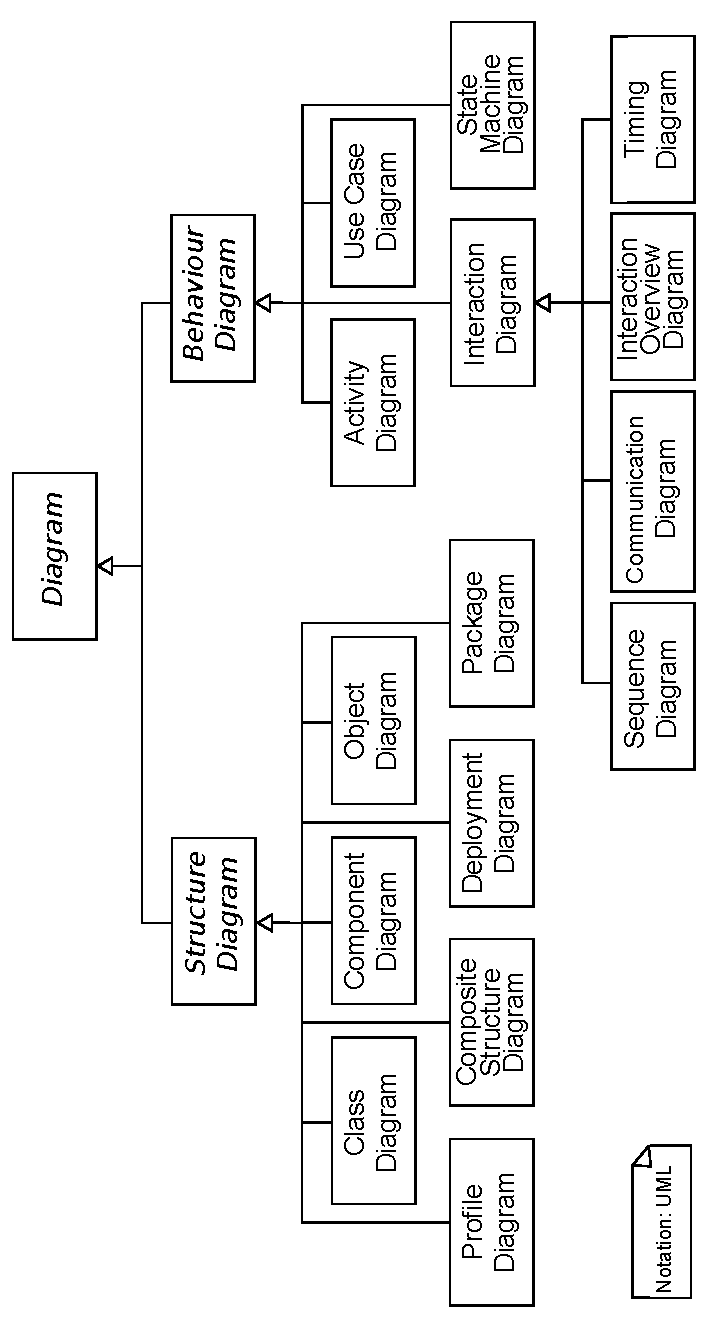
\includegraphics[scale=0.3,angle=270]{images/uml}
 \caption{\textit{UML} diagram type hierarchy (Derfel73, PMerson)}
 \label{fig:uml}
\end{figure}
\end{frame}

\begin{frame}
\frametitle{UML Models and Refactoring}
\begin{itemize}
 \item Whats the difference between source code and model refactoring?
 \begin{itemize}
  \item Consider all interconnected views/diagrams
  \item Consider model constraints
  \item Consider different abstraction levels
    \begin{itemize}
	\item Not all aspects fully modeled
    \end{itemize}
 \end{itemize}
 \item Example:
\begin{itemize}
 \item In Java fields and methods are directly in one class
 \item In UML Activities are modeled separate from Classes
\end{itemize}
\end{itemize}        
\end{frame}


\begin{frame}
\frametitle{Semantic Preservation}
\begin{itemize}
 \item How to preserve semantics and verify models?
 \begin{itemize}
  \item Static analysis: Specify pre- and postconditions with OCL constraints
  \item Validate refactored models.
  \item Dynamics analysis: Execute models and analyse behavior and execution properties (trace).
 \end{itemize} 
\item What means semantic preservation?
 \begin{itemize}
  \item Same execution trace?
  \item Same output?
  \item Same state?
 \end{itemize}
 \item Depends on refactoring!
\end{itemize}
\end{frame}

\begin{frame}
\frametitle{Insurance Company Example 1/3}
\begin{figure}[h!t]
 \centering
 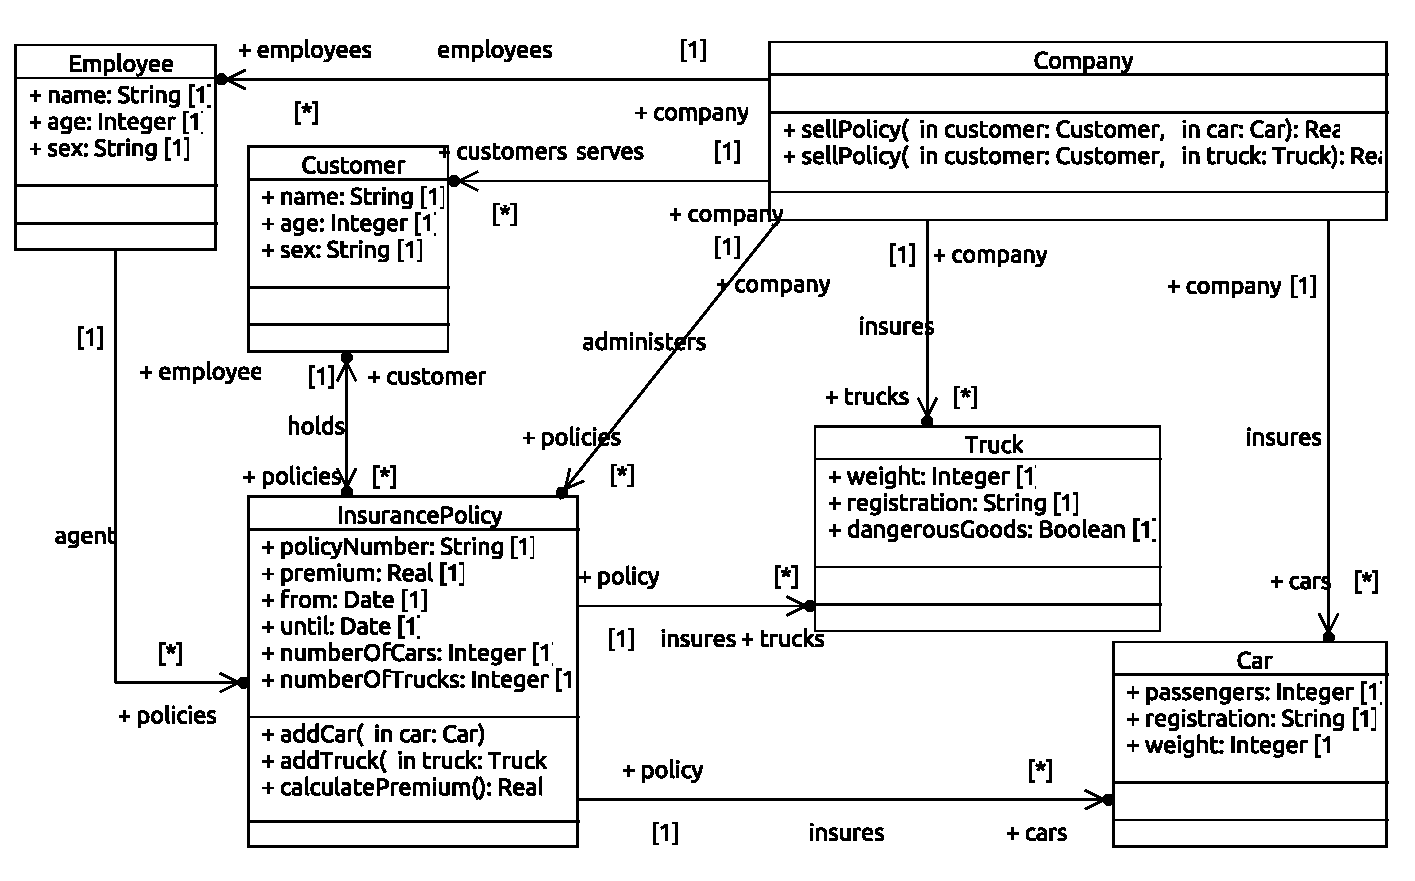
\includegraphics[scale=0.4]{images/insurance/Model_Model_ClassDiagram}
 \caption{Insurance class diagram}
 \label{fig:classdiagramcomplexRef}
\end{figure}
\end{frame}

        
\begin{frame}
\frametitle{Insurance Company Example 2/3}
\begin{figure}[h!t]
 \centering
 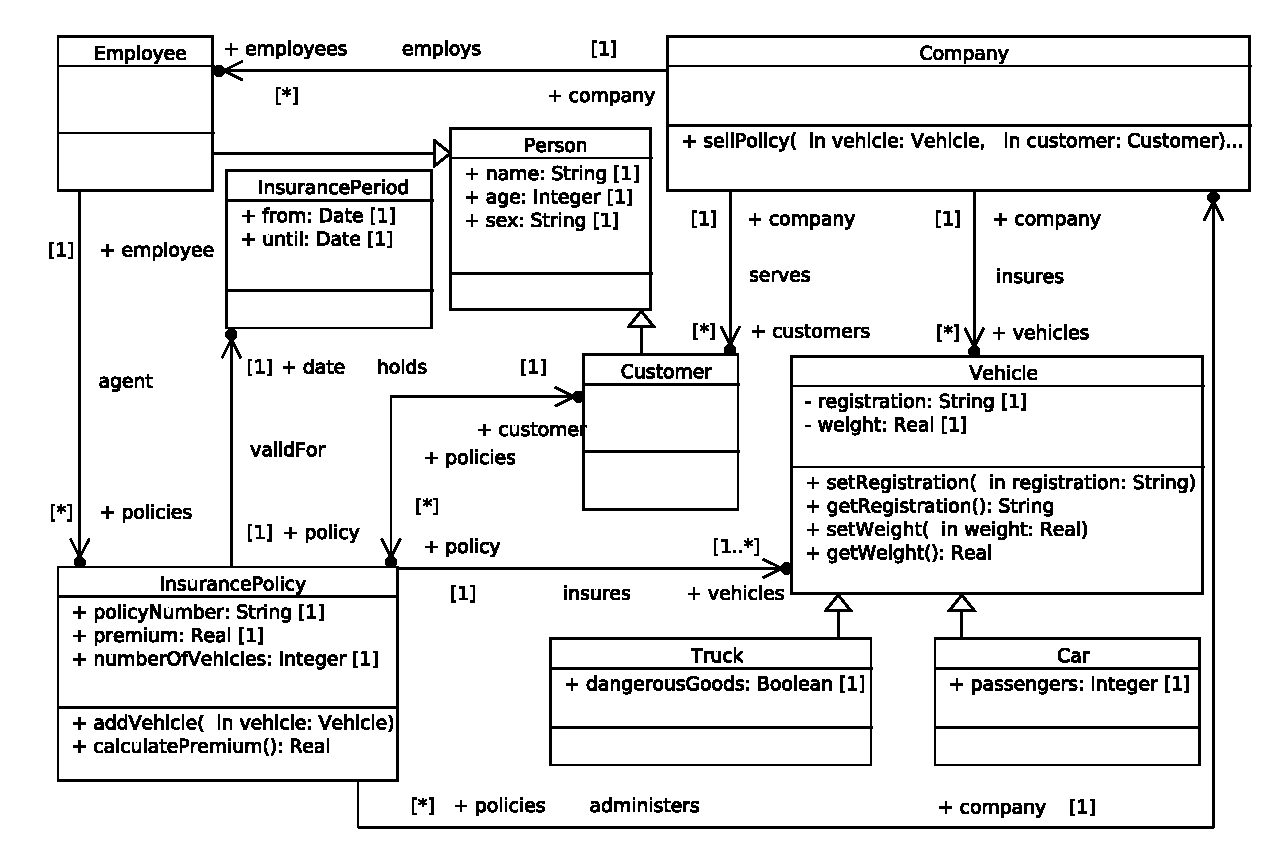
\includegraphics[scale=0.4]{images/insurance_ref/Model_Model_ClassDiagram}
 \caption{Insurance class diagram with refactorings}
 \label{fig:classdiagramcomplex}
\end{figure}
\end{frame}

\begin{frame}
\frametitle{Insurance Company Example 3/3}
\begin{figure}[h!t]
 \centering
 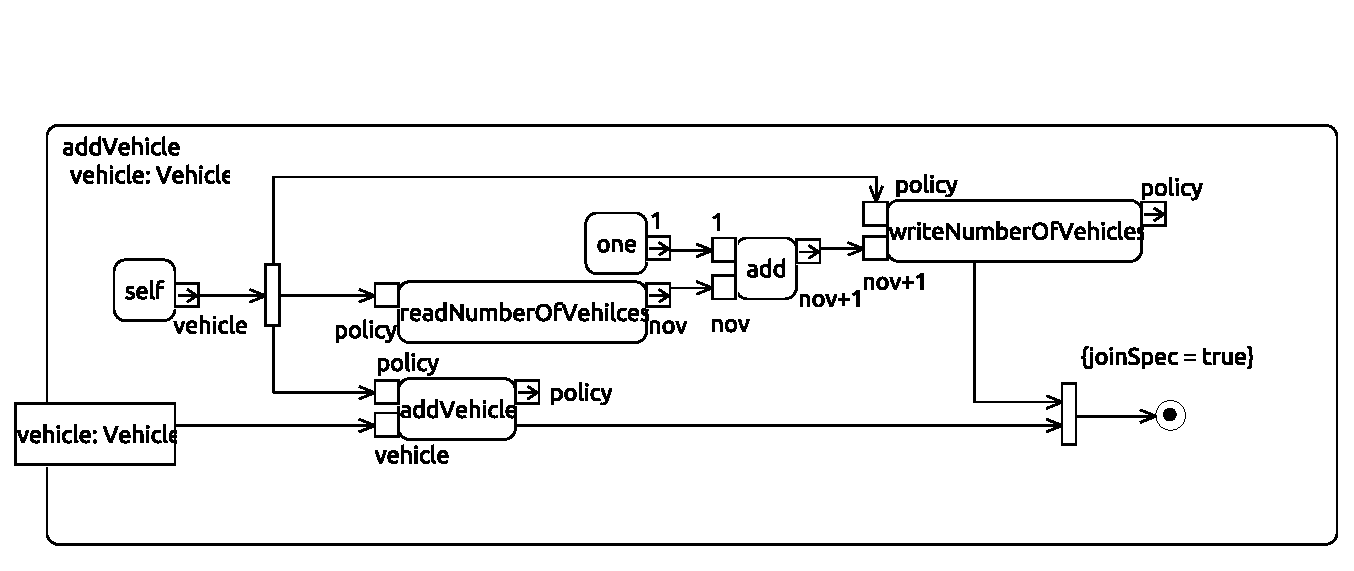
\includegraphics[scale=0.45]{images/insurance_ref/Activity_addVehicle_addVehicle}
 \caption{Add vehicle activity}
 \label{fig:calculatePremium}
\end{figure}
\end{frame}




\begin{frame}
\frametitle{fUML Introduction}
\begin{itemize}
 \item fUML = foundational UML \cite{man:FUML}
 \item fUML 1.1 is based on UML 2.4.1
 \item Subset of UML (Class and Activity diagrams)
 \item Enhanced with consise semantics
 \item Turing complete and allows execution or interpretation
 \item Existing VM to execute models
 \item Extended VM for testing and debugging (Moliz) \cite{DBLP:conf/models/MayerhoferLK12}
\end{itemize}
\end{frame}

\begin{frame}
\frametitle{fUML Abstract Syntax for Classifiers}
\begin{figure}[h!t]
 \centering
 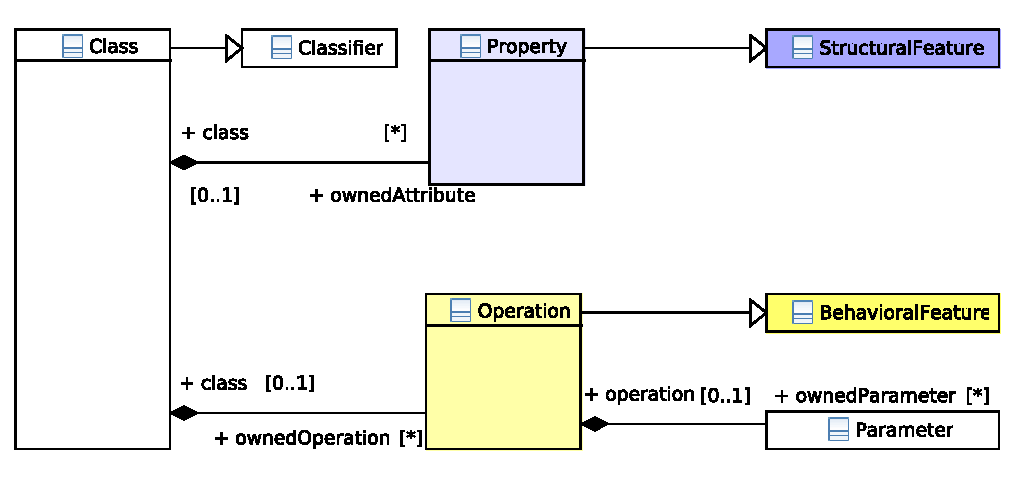
\includegraphics[scale=0.5]{images/Model_Model_Classifiers_pres}
 \caption{Classifiers in fUML}
 \label{fig:classifiers}
\end{figure}
\end{frame}


\begin{frame}
 \frametitle{fUML Actions}
 Actions provide the functionality of activity diagrams. Every behavior is based on an action.
 \begin{itemize}
  \item ReadSelfAction
  \item AddStructuralFeatureValueAction
  \item RemoveStructuralFeatureValueAction
  \item ReadStructuralFeatureAction
  \item WriteStructuralFeatureAction
  \item ValueSpecification
 \end{itemize}
\begin{figure}[h!t]
 \centering
 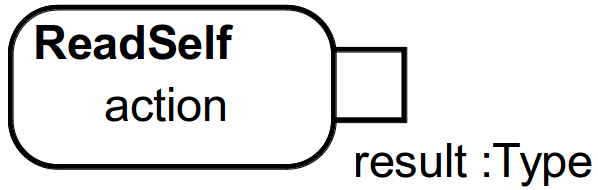
\includegraphics[scale=0.18]{images/fuml-actions/ReadSelf.png}
\end{figure}
\end{frame}

\begin{frame}
\frametitle{fUML Actions (2)}
\begin{figure}[h!t]
 \centering
 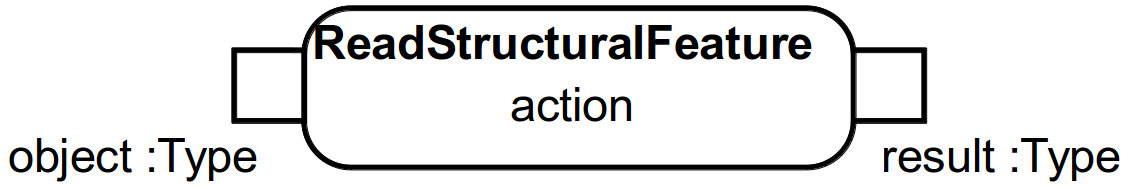
\includegraphics[scale=0.18]{images/fuml-actions/ReadStructuralFeature.png}
\end{figure}
\begin{figure}[h!t]
 \centering
 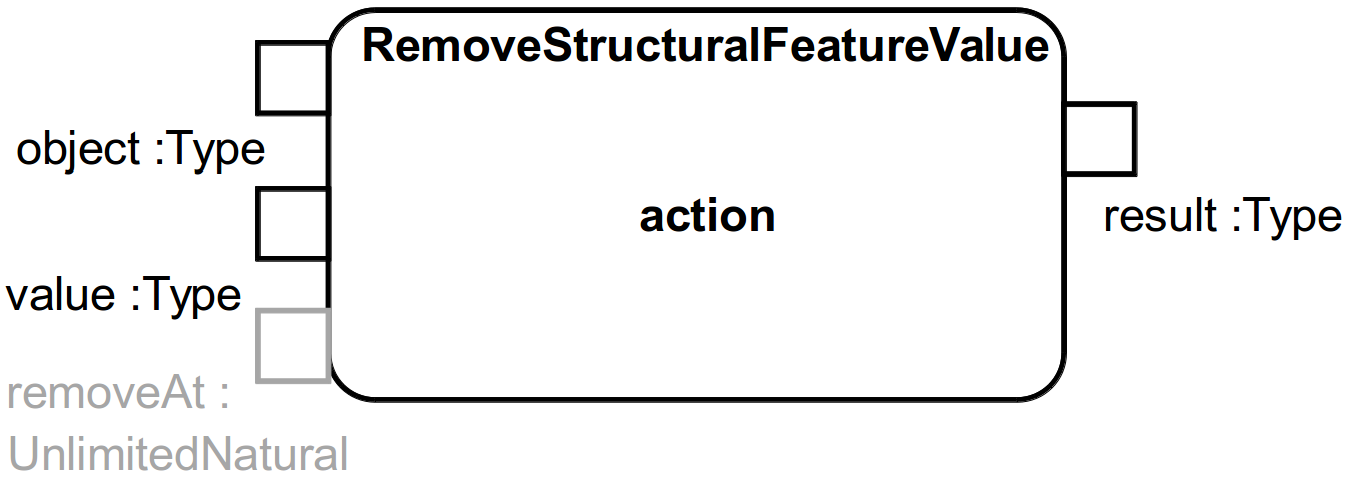
\includegraphics[scale=0.18]{images/fuml-actions/RemoveStructuralFeatureValue.png}
\end{figure}
\begin{figure}[h!t]
 \centering
 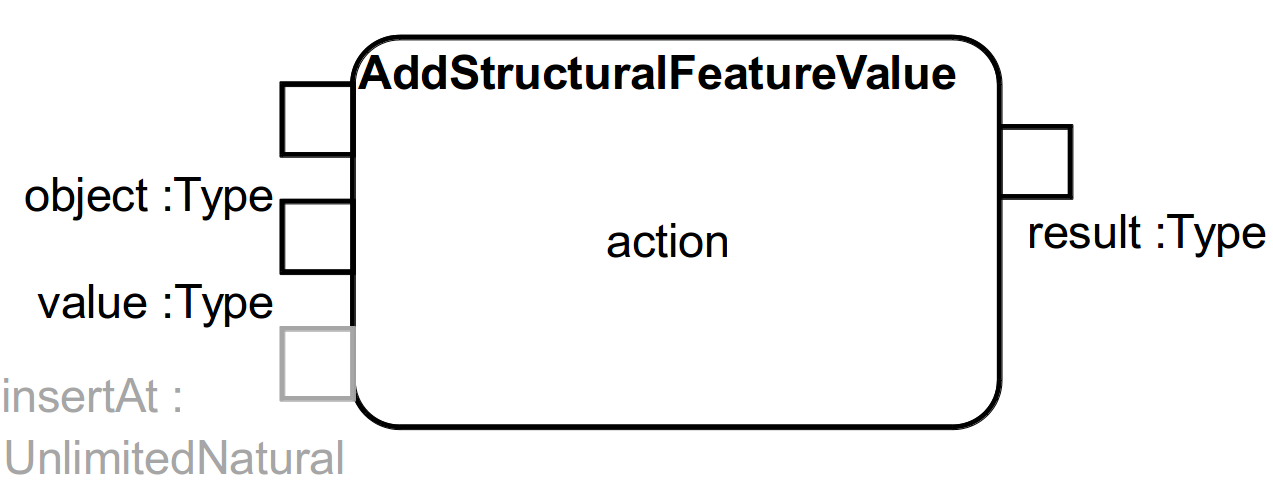
\includegraphics[scale=0.18]{images/fuml-actions/AddStructuralFeatureValue.png}
\end{figure}
\end{frame}

\begin{frame}
 \frametitle{fUML Actions (3)}
\begin{figure}[h!t]
 \centering
 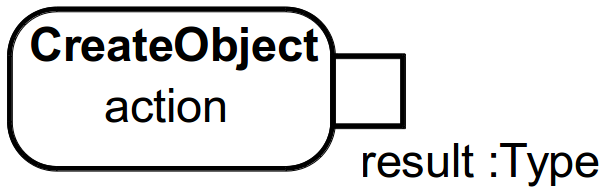
\includegraphics[scale=0.18]{images/fuml-actions/CreateObject.png}
\end{figure}
\begin{figure}[h!t]
 \centering
 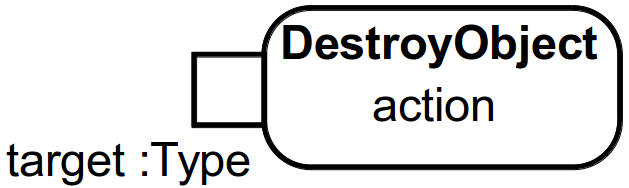
\includegraphics[scale=0.18]{images/fuml-actions/DestroyObject.png}
\end{figure}
\begin{figure}[h!t]
 \centering
 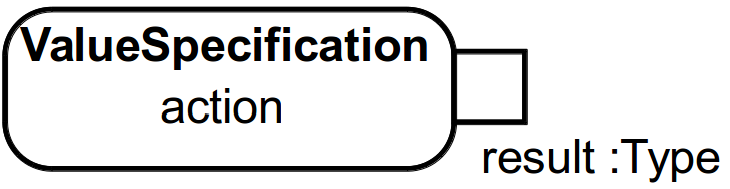
\includegraphics[scale=0.18]{images/fuml-actions/ValueSpecification.png}
\end{figure}
\end{frame}

\begin{frame}
\frametitle{fUML Abstract Syntax for Actions}
\begin{figure}[h!t]
 \centering
 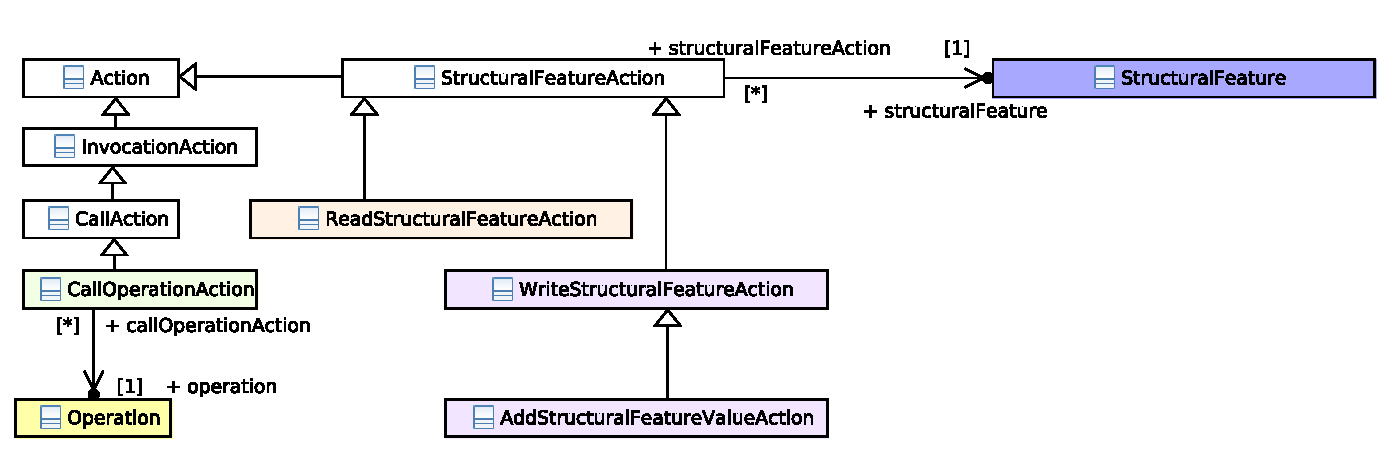
\includegraphics[scale=0.5]{images/Model_Model_Behavior_pres}
 \caption{Actions in fUML}
 \label{fig:behavior}
\end{figure}
\end{frame}

        
%USE 2-3 slides for this!
\begin{frame}
\frametitle{Encapsulate Field Prerefactoring}
Public field (property) \textbf{policyNumber}:
\begin{figure}
 \centering
 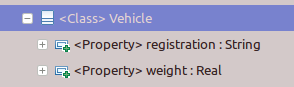
\includegraphics[scale=0.35]{images/fuml-refactorings/vehicle-prerefactoring.png}
\end{figure}
\end{frame}

\begin{frame}
 \frametitle{Encapsulate Field Postrefactoring}
Property is private, operations and activities have been added:
\begin{figure}
 \centering
 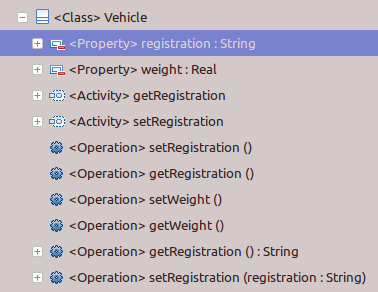
\includegraphics[scale=0.35]{images/fuml-refactorings/vehicle-postrefactoring.png}
\end{figure}
The activity for the getter:
\begin{figure}
 \centering
 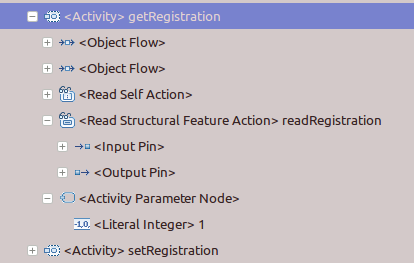
\includegraphics[scale=0.35]{images/fuml-refactorings/vehicle-getter-activity.png}
\end{figure}

\end{frame}

        
\begin{frame}[fragile]
\frametitle{Refactoring Constraints with OCL}
Constraint ensure that the model is in a good state
before and after the refactoring.

Example:
\begin{lstlisting}[morekeywords={self,forAll,uml,VisibilityKind,o}]
context Property:
pre : self.visibility <> 
          uml::VisibilityKind::private and 
      self.class.ownedOperation
      ->forAll(o | o.isDistinguishableFrom(
           setOperation, 
           self.namespace) and
      o.isDistinguishableFrom(getOperation,
                              self.namespace))
\end{lstlisting}

\end{frame}

\begin{frame}[fragile]
\frametitle{Refactoring Constraints with OCL}
Constraint for searching parts of the model that need to be adapted.

Example:
\begin{lstlisting}[morekeywords={self,forAll,uml,VisibilityKind,o,oclAsType,oclIsTypeOf}]
context Package:
self.member->select(c|c.oclIsTypeOf(Class)).
    oclAsType(Class).member->
    select(a|a.oclIsTypeOf(Activity)).
    oclAsType(Activity).node->
    select(n|n.oclIsTypeOf(
    ReadStructuralFeatureAction)).
    oclAsType(ReadStructuralFeatureAction).
    structuralFeature
\end{lstlisting}

\end{frame}

\begin{frame}
\frametitle{Toolchain}
\begin{itemize}
 \item Used Eclipse Modeling Framework and Ecore
 \item Java implementation of UML 2.4.1 (org.eclipse.uml2.uml)
 \item Created constraints with Eclipse OCL Console
 \item Evaluate constraints with OCL Java API (org.eclipse.ocl)
 \item Model transformation is performed through UML's abstract syntax.
\end{itemize}
\end{frame}

\begin{frame}
\frametitle{Toolchain}
 \begin{figure}[h!t]
 \centering
 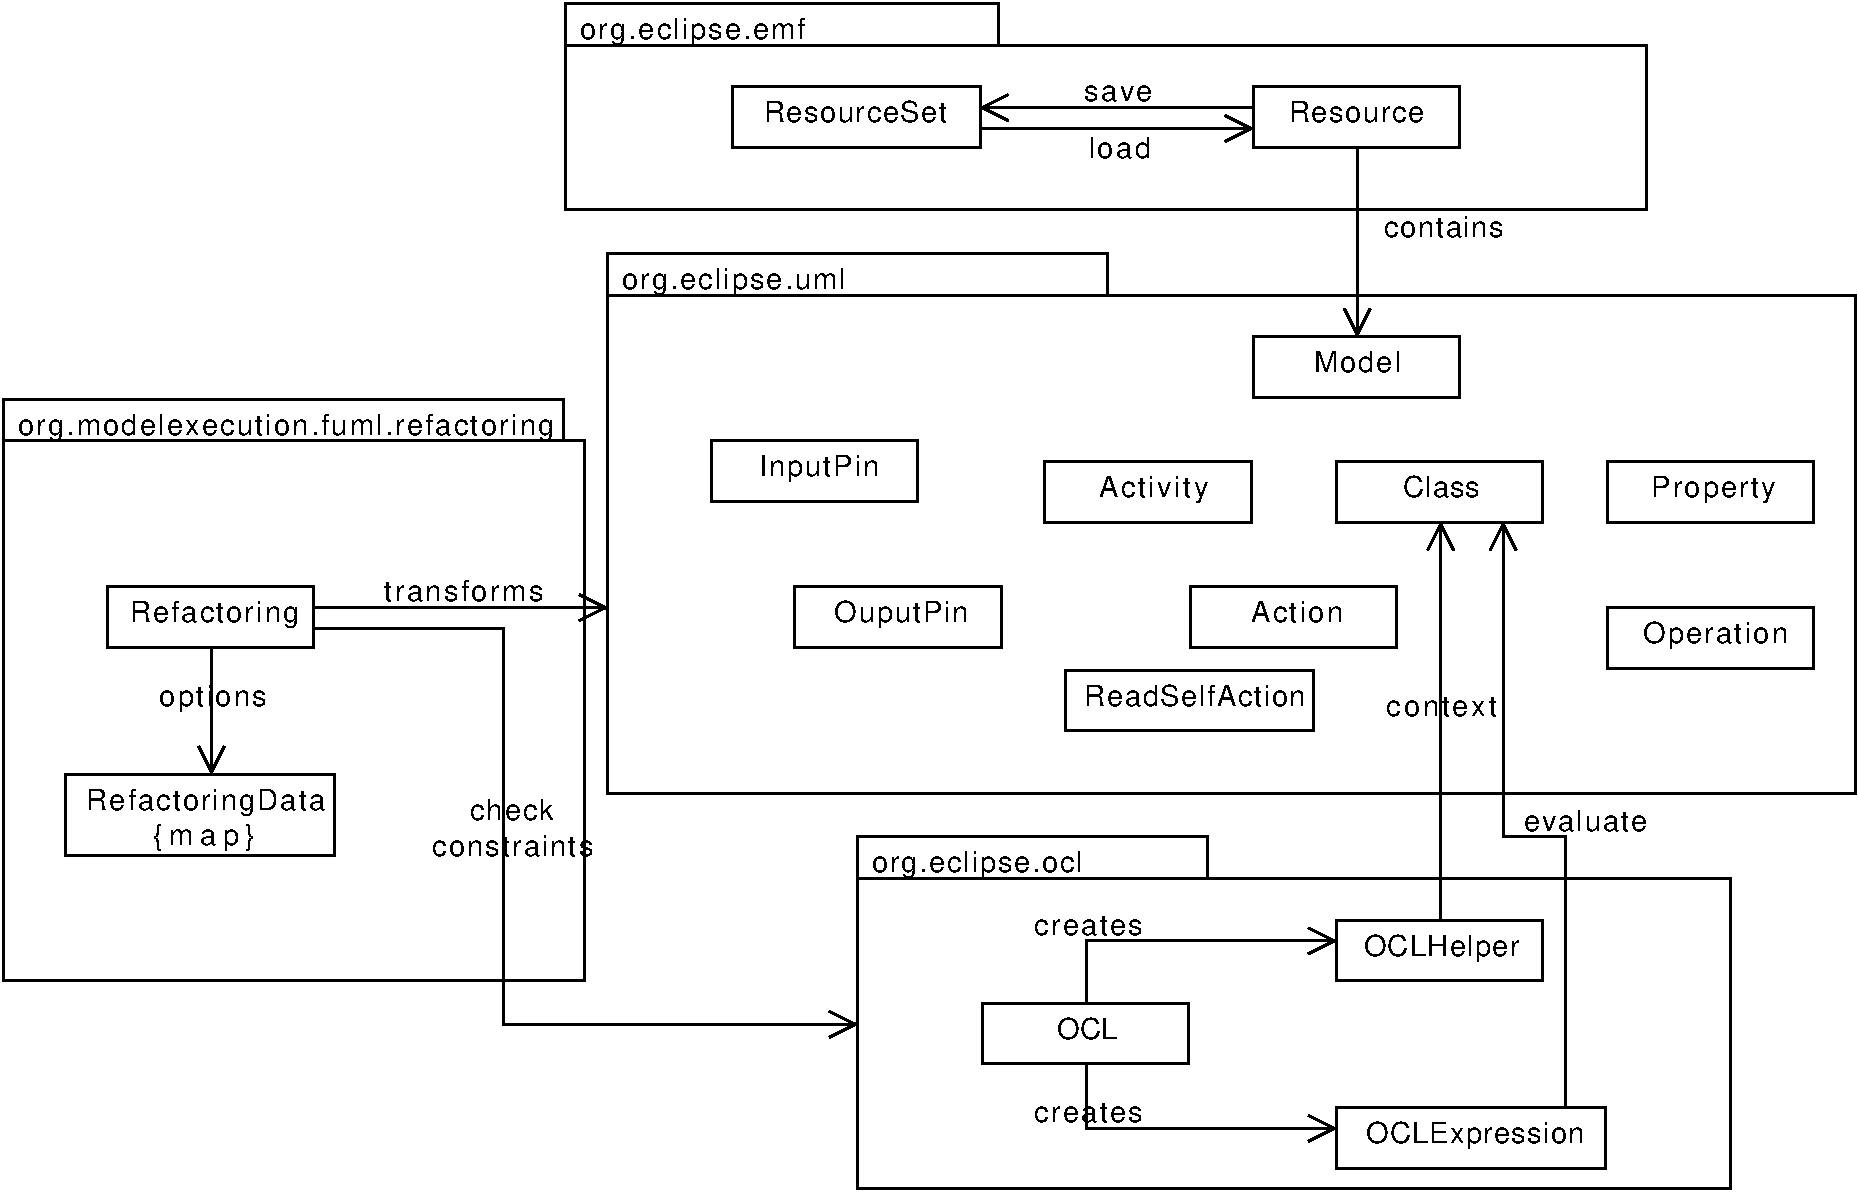
\includegraphics[scale=0.35]{figures/Toolchain2}
\end{figure}
\end{frame}

        
\begin{frame}
\frametitle{EMF Refactor}
\begin{itemize}
 \item Framework for Eclipse to
 \begin{itemize}
  \item check for ``model smells'' and show metrics (e.g. complexity)
  \item refactor models and their properties
  \item define your own refactorings/metrics
 \end{itemize}
 \item Suggests refactorings based on metrics
 \item Generates new stubs for Java, OCL, Henshin and ComRel
 \item Is Gui/Wizard based and works for
 \begin{itemize}
  \item Papyrus
  \item EMF Treeeditor
 \end{itemize}

\end{itemize}

\end{frame}
        

\begin{frame}
 \begin{center}
\Huge Questions?
\end{center}
\end{frame}

\begin{frame}
 \frametitle{References}
 \bibliographystyle{acm}
 \bibliography{references}
\end{frame}

\end{document}
